\documentclass[12pt]{article}
\usepackage{amsmath}
\usepackage{amssymb}
\usepackage{tikz}
\usepackage{geometry}
\usepackage{graphicx}
\geometry{a4paper, margin=1in}

\author{}
\date{}
\title{Introduction to Sets\\Course\\
\vspace{28pt}
\begin{center}

\includegraphics[width=4em]{ApS_logo.png}
\end{center}
\begin{normalsize}Tutoring Centre Ferndale\end{normalsize}}

\begin{document}

\maketitle

Sets are collections of objects. A knowledge of sets forms the foundation for many areas of mathematics and is essential for understanding more advanced topics.

\section{Definitions and Symbols}

\begin{itemize}
    \item \(\emptyset\): The empty set, a set with no elements.
    \item \(\in\): Symbol for "is an element of." For example, \(a \in A\) means \(a\) is an element of set \(A\).
    \item \(\notin\): Symbol for "is not an element of." For example, \(b \notin B\) means \(b\) is not an element of set \(B\).
    \item \(\subset\): Symbol for "is a subset of." For example, \(A \subset B\) means every element of \(A\) is also an element of \(B\).
    \item \(\cup\): Union of two sets. \(A \cup B\) is the set of elements in either \(A\) or \(B\) or both.
    \item \(\cap\): Intersection of two sets. \(A \cap B\) is the set of elements in both \(A\) and \(B\).
    \item \(\setminus\): Difference between two sets. \(A \setminus B\) is the set of elements in \(A\) but not in \(B\).
    \item \(\mathbb{N}\): The set of natural numbers \(\{1, 2, 3, \ldots\}\).
    \item \(\mathbb{Z}\): The set of integers \(\{\ldots, -2, -1, 0, 1, 2, \ldots\}\).
    \item \(\mathbb{Q}\): The set of rational numbers (fractions).
    \item \(\mathbb{R}\): The set of real numbers.
\end{itemize}

\newpage

\section{Venn Diagrams}

Venn diagrams are a way to visually represent sets and their relationships.

\begin{center}
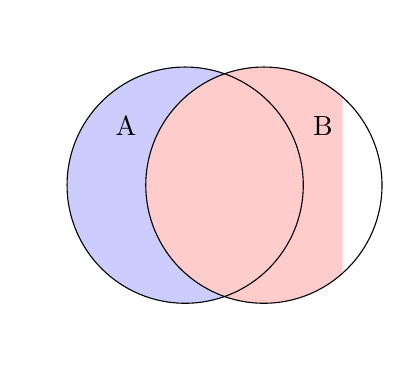
\begin{tikzpicture}
    \begin{scope}
        \clip (-2,-2) rectangle (2,2);
        \fill[blue!20] (0,0) circle (1.5);
        \fill[red!20] (1,0) circle (1.5);
    \end{scope}
    \draw (0,0) circle (1.5);
    \draw (1,0) circle (1.5);
    \node at (-0.75, 0.75) {A};
    \node at (1.75, 0.75) {B};
\end{tikzpicture}
\end{center}

In the Venn diagram above:
\begin{itemize}
    \item The blue area represents set \(A\).
    \item The red area represents set \(B\).
    \item The purple area represents the intersection \(A \cap B\).
    \item The combined areas represent the union \(A \cup B\).
\end{itemize}

\newpage

\section{Exercises}

\subsection*{Question 1}

Given the sets \(A = \{1, 2, 3, 4\}\) and \(B = \{3, 4, 5, 6\}\), find \(A \cup B\), \(A \cap B\), and \(A \setminus B\).

\subsection*{Answer 1}

\begin{itemize}
    \item \(A \cup B = \{1, 2, 3, 4, 5, 6\}\)
    \item \(A \cap B = \{3, 4\}\)
    \item \(A \setminus B = \{1, 2\}\)
\end{itemize}

\subsection*{Question 2}

Draw a Venn diagram for the sets \(A = \{1, 2, 3\}\), \(B = \{3, 4, 5\}\), and \(C = \{5, 6, 7\}\). Shade the region representing \(A \cap (B \cup C)\).

\subsection*{Answer 2}

\begin{center}
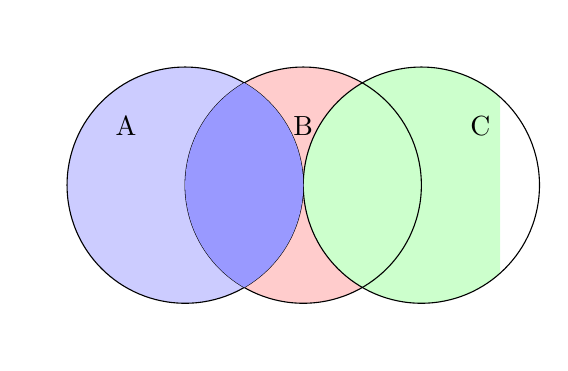
\begin{tikzpicture}
    \begin{scope}
        \clip (-2,-2) rectangle (4,2);
        \fill[blue!20] (0,0) circle (1.5);
        \fill[red!20] (1.5,0) circle (1.5);
        \fill[green!20] (3,0) circle (1.5);
    \end{scope}
    \draw (0,0) circle (1.5);
    \draw (1.5,0) circle (1.5);
    \draw (3,0) circle (1.5);
    \node at (-0.75, 0.75) {A};
    \node at (1.5, 0.75) {B};
    \node at (3.75, 0.75) {C};
    % Shade the intersection of A and (B union C)
    \begin{scope}
        \clip (0,0) circle (1.5);
        \fill[blue!40] (1.5,0) circle (1.5);
        \fill[blue!40] (3,0) circle (1.5);
    \end{scope}
\end{tikzpicture}
\end{center}

\subsection*{Explanation}

The region representing \(B \cup C\) is the union of the red and green circles. The intersection \(A \cap (B \cup C)\) is where the blue circle overlaps with this union.

\subsection*{Question 3}

If \(U = \{1, 2, 3, 4, 5, 6, 7, 8, 9\}\) is the universal set, and \(A = \{2, 4, 6, 8\}\), find the complement of \(A\), denoted \(A^c\).

\subsection*{Answer 3}

The complement of \(A\) is the set of elements in \(U\) that are not in \(A\):

\[
A^c = \{1, 3, 5, 7, 9\}
\]

\subsection*{Explanation}

The universal set \(U\) contains all elements under consideration. The complement of \(A\) includes all elements of \(U\) that are not in \(A\).

\end{document}
